\section{PnP step by step, with the real camera}\label{sec:pnp-steps}

This section answers, with numbers, the questions ``what exactly is computed when the drone sees a marker'',
``why four corners and not the centre'', ``what is this mirror ambiguity'' and ``why a solver''. All numbers use the
real calibration of \file{config/tello\_camera.yaml} ($f_x = 910.47$, $f_y = 913.55$, $c_x = 466.65$,
$c_y = 363.89$~px), without distortion for clarity. They are produced by \file{docs/book/figures/pnp\_example.py}.

\begin{keypoint}
\textbf{This is not epipolar geometry.} Epipolar geometry (epipolar plane, essential matrix $E$) relates
\emph{two images} of the same unknown 3D point. Here there is \emph{one} image and points whose 3D position is
\emph{already known} (the marker corners, from \file{markers.yaml}). The problem is Perspective-n-Point: find
where the camera is so that the known 3D points fall on the measured pixels.
\end{keypoint}

\subsection{What is known, what is unknown}

\begin{center}
\begin{tabular}{@{}lll@{}}
\toprule
& What & Where it comes from \\
\midrule
known & 3D position $P_k$ of every corner, in \code{map} & \file{markers.yaml} (centre $t_m$, axes $R_m$, side $\ell$) \\
known & pixel $p_k = (u_k, v_k)$ of every corner & the detector (sub-pixel corners) \\
known & $K$, $D$ & the calibration \\
\textbf{unknown} & \textbf{one} rotation $R$ and \textbf{one} translation $t$ & what PnP solves \\
\bottomrule
\end{tabular}
\end{center}

The unknown is \emph{not} ``one transformation per point''. It is a single rigid transformation, the pose of the
camera, that is the same for all the points: a corner $P_k$ of the room is seen in the camera frame at
\begin{equation}
P_k^{c} = R\,P_k + t = \begin{bmatrix} X_k \\ Y_k \\ Z_k \end{bmatrix}
\qquad\text{(camera frame: $x$ right, $y$ down, $z$ forward)}.
\end{equation}
$R$ has 3 degrees of freedom and $t$ has 3: \textbf{6 unknown numbers in total}, whatever the number of points.
The points are the \emph{measurements} that pin these 6 numbers down.

\subsection{Perspective = dividing by the depth}

A point in front of the camera lands on the pixel
\begin{equation}
u = f_x \frac{X}{Z} + c_x, \qquad v = f_y \frac{Y}{Z} + c_y .
\label{eq:pinhole}
\end{equation}
That division by $Z$ \emph{is} perspective: the same object twice as far is half as big in the image.

\paragraph{Example 1: a marker facing the camera.} Its corners are at $X, Y = \pm\ell/2 = \pm 0.0945$~m. At
$Z = 2$~m: $u = 910.47 \times (\pm 0.0945)/2 + 466.65 = 509.6$ or $423.7$, so the marker is $86.0$~px wide. At
$Z = 1$~m it is $172.0$~px wide. The size gives the distance:
$d = f_x \ell / (\text{width in px}) = 910.47 \times 0.1889 / 86.0 = 2.00$~m. This is exactly the formula of
\topic{/aruco/nearest\_marker}.

\paragraph{Example 2: the same marker turned by $20^\circ$.} Now one vertical edge is closer to the camera than the
other ($Z$ differs by $\ell\sin 20^\circ = 6.5$~cm). The closer edge looks taller, the far one shorter, and the
marker looks narrower: the square becomes a \emph{trapezoid}.

\begin{center}
\begin{tabular}{@{}lccc@{}}
\toprule
Marker at 2 m & width (px) & left edge (px) & right edge (px) \\
\midrule
facing the camera & 86.0 & 86.3 & 86.3 \\
turned $+20^\circ$ & 80.8 & 84.9 & 87.7 \\
turned $-20^\circ$ & 80.8 & 87.7 & 84.9 \\
\bottomrule
\end{tabular}
\end{center}

The width shrinks by $\cos 20^\circ$ (it tells \emph{how much} the marker is turned), and the difference between the two
edges (here $2.8$~px) tells \emph{which way}. That is the whole ``perspective transformation'': the shape of the
quadrilateral in the image encodes the angle, its size encodes the distance, its position in the image encodes the
direction.

\begin{figure}[h]
\centering
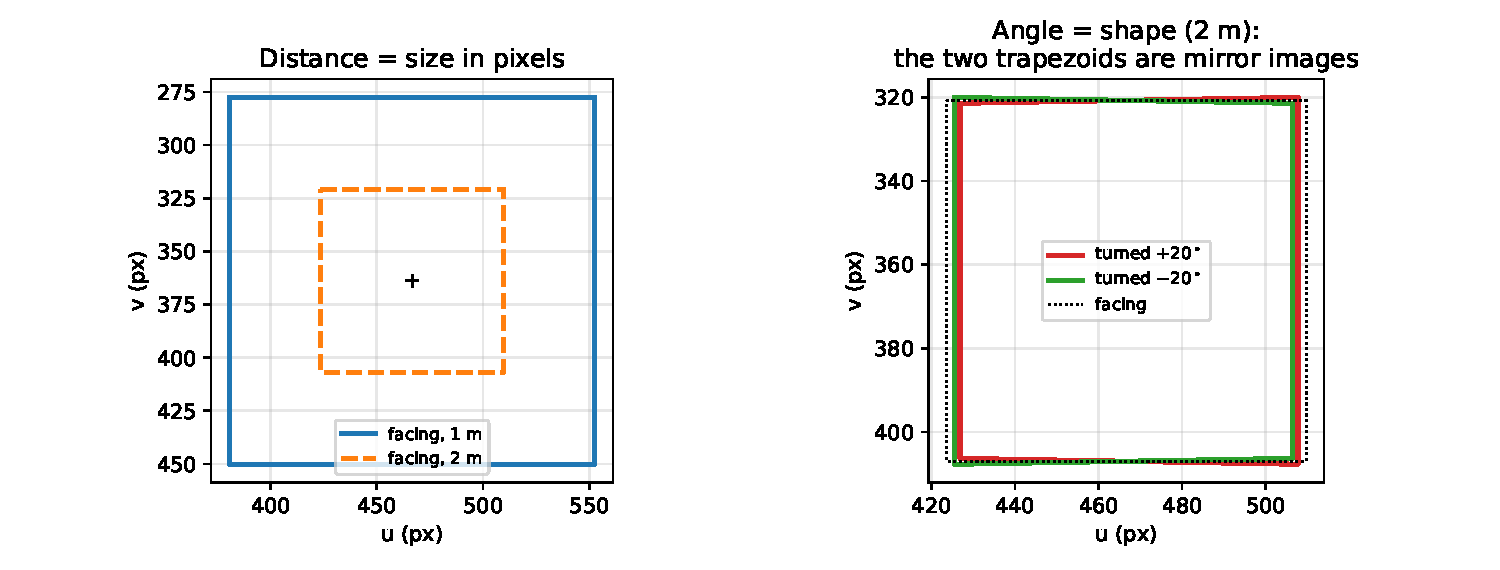
\includegraphics[width=\textwidth]{figures/pnp_perspective.pdf}
\caption{Left: distance = size (1 m vs 2 m). Right: angle = shape. Turned $+20^\circ$ and $-20^\circ$ give mirror
trapezoids that differ by only $\approx 1.4$~px per corner.}
\end{figure}

\subsection{Counting equations: why four corners and not the centre}

Each pair ``known 3D point $\leftrightarrow$ measured pixel'' gives \textbf{2 equations} (its $u$ and its $v$,
eq.~\ref{eq:pinhole}). There are \textbf{6 unknowns}.

\begin{center}
\begin{tabular}{@{}lll@{}}
\toprule
Points used & Equations & What it fixes \\
\midrule
centre of 1 marker & 2 & only a \emph{ray}: the camera is somewhere on the line through the marker centre \\
2 points & 4 & a one-parameter family of poses \\
3 points & 6 & a finite set: up to 4 poses (the classical P3P problem) \\
4 corners of 1 marker & 8 & one pose in theory, but two nearly equivalent in practice (next subsection) \\
4 corners of $n \geq 2$ markers & $8n$ & one well-determined pose \\
\bottomrule
\end{tabular}
\end{center}

With centres only, the drone would need at least three markers in view at the same time to compute anything, and
it would throw away the size and shape of each marker (the distance and angle information of the examples above).
The four corners carry all of it, so one marker is already enough.

\paragraph{Several markers: one problem.} All corners of all visible markers are expressed in the same \code{map}
frame, so they are simply stacked: 3 markers give 12 pairs and 24 equations for the same 6 unknowns. The angle
gets much better because the points are spread out: the angle error is roughly (pixel error) / (pixel distance
between the points). For a corner error of $0.5$~px at 2~m: one marker (corners $86$~px apart) gives
$0.5/86 = 0.006$~rad $= 0.33^\circ$; two markers 1~m apart ($455$~px) give $0.06^\circ$. It is like measuring a slope
with a long ruler instead of a short one.

\subsection{The mirror ambiguity of a single marker}

A 19~cm marker seen from 1--3~m is small compared with its distance. The perspective effect that tells
``turned left'' from ``turned right'' is then tiny: in the table above, turning the marker $+20^\circ$ or $-20^\circ$
changes each corner by only about $1.4$~px, and the detector's corners have $\approx 0.3$~px of noise. Two camera
poses explain the 4 corners almost equally well. In the map they are symmetric about the line of sight: the camera
is either to the left or to the right of the marker's normal.

\paragraph{Example 3: what OpenCV returns.} Marker $0.5$~m to the right of the optical axis, 2~m away, turned
$20^\circ$; $0.3$~px of noise on the corners; \code{solvePnPGeneric(..., SOLVEPNP\_IPPE\_SQUARE)} returns:
\begin{center}
\begin{tabular}{@{}lcc@{}}
\toprule
& reprojection error & camera position in the marker frame (m) \\
\midrule
solution 1 & 0.21 px & $(+0.30,\ -0.07,\ 2.03)$ \\
solution 2 & 0.33 px & $(-0.30,\ +0.07,\ 2.03)$ \\
\bottomrule
\end{tabular}
\end{center}
Both explain the pixels to a third of a pixel, yet the two camera positions are \textbf{0.62~m apart}. The ratio of the
errors is $0.33/0.21 = 1.6 < 3$, so \code{single\_marker\_pose} does not trust the best one blindly: it takes the one
closest to the last pose (less than 1~s old and 0.4~m away), and otherwise rejects the image. With two markers or
more the two solutions no longer exist: the points are spread out and not on one small plane.

\begin{figure}[h]
\centering
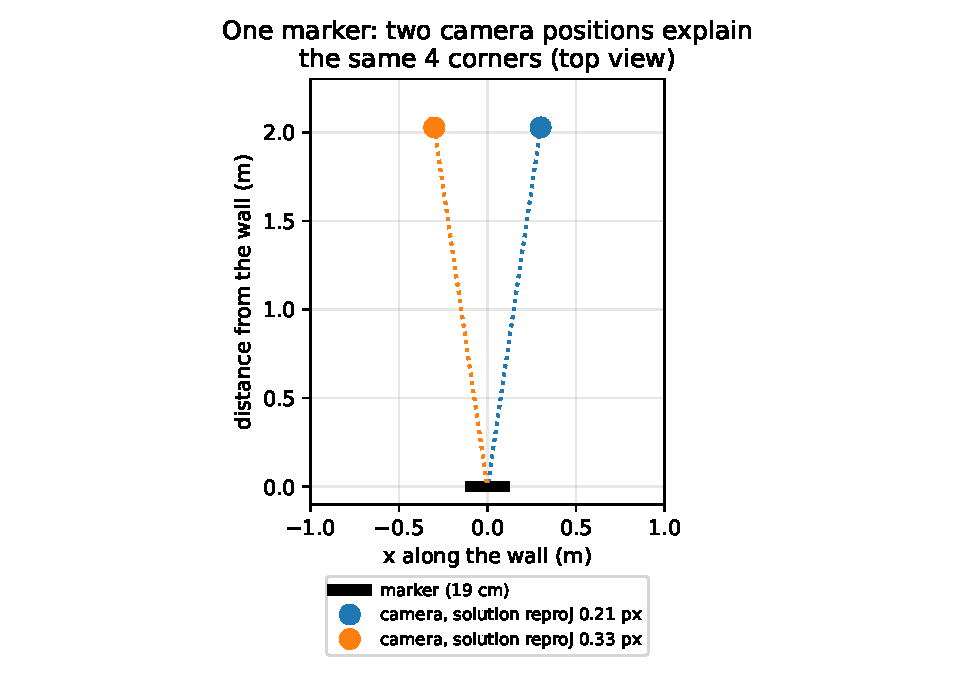
\includegraphics[width=0.55\textwidth]{figures/pnp_mirror.pdf}
\caption{Example 3, top view: two camera positions, 0.62~m apart, explain the same four corners to $0.2$--$0.3$~px.}
\end{figure}

\subsection{Why a solver, and not a formula}

Write eq.~\ref{eq:pinhole} for one corner with the unknowns visible ($r_1^\top, r_2^\top, r_3^\top$ are the rows of
$R$):
\begin{equation}
u_k = f_x \frac{r_1^\top P_k + t_x}{r_3^\top P_k + t_z} + c_x, \qquad
v_k = f_y \frac{r_2^\top P_k + t_y}{r_3^\top P_k + t_z} + c_y .
\end{equation}
Three things make it non-linear, even without any noise:
\begin{enumerate}[leftmargin=*]
\item the unknowns are in a \textbf{fraction} (the division by the depth);
\item $R$ must be a \textbf{rotation}: $R^\top R = I$, $\det R = 1$, i.e.\ 6 quadratic constraints on its 9 entries;
\item the lens \textbf{distortion} $D$ adds polynomial terms ($k_1 r^2 + k_2 r^4 + \dots$) before the pixel.
\end{enumerate}
On top of this, the measurements are noisy: no pose satisfies all the equations exactly, so we look for the pose
that makes the total pixel error as small as possible (least squares):
\begin{equation}
\min_{R,\,t} \; \sum_k \big\lVert \pi(K, D, R P_k + t) - p_k \big\rVert^2 .
\label{eq:pnp-ls}
\end{equation}

\paragraph{The linear shortcut (DLT) and why it is not enough.} Multiplying out the fraction gives equations that are
\emph{linear} in the 12 entries of $M = K[R \mid t]$:
\begin{equation}
(u_k - c_x)\,(r_3^\top P_k + t_z) - f_x\,(r_1^\top P_k + t_x) = 0 .
\end{equation}
Stacking them and taking the SVD solves for $M$ in one shot. But the solution ignores the rotation constraint (the
$R$ found is not a rotation and must be ``straightened'', which adds error), it minimises this algebraic residual and
not the pixel error, it ignores the distortion, and it degenerates when all points are on one plane (one marker). For
a planar marker the linear tool is the \emph{homography} $H \simeq K[r_1\ r_2\ t]$ between the square and the image, which
4 corners determine exactly; IPPE starts from it.

\paragraph{What the code does.}
\begin{center}
\begin{tabular}{@{}p{3.2cm}p{5.6cm}p{5.2cm}@{}}
\toprule
Solver & What it does & When \\
\midrule
\code{IPPE\_SQUARE} & from the homography of one square, returns \emph{both} candidate poses analytically & one marker in view \\
\code{SQPNP} & global minimum of eq.~\ref{eq:pnp-ls} (without distortion) over true rotations, no initial guess & two markers or more \\
\code{solvePnPRefineLM} & Levenberg--Marquardt on eq.~\ref{eq:pnp-ls} with distortion, from the previous solution & always, after the two others \\
\bottomrule
\end{tabular}
\end{center}
One Levenberg--Marquardt step linearises the residuals $r(x)$ (stacked pixel errors, $x$ = the 6 pose parameters,
$J$ = their Jacobian) and moves by
\begin{equation}
\delta x = -\left(J^\top J + \mu I\right)^{-1} J^\top r ,
\end{equation}
a Gauss--Newton step when $\mu$ is small, a small gradient step when $\mu$ is large; a few iterations are enough from the
IPPE/SQPnP start. The error left at the end, the RMS reprojection error, is the quality check: a pose is rejected above
$3$~px with one marker and above $8$~px with several (a marker moved since the mapping, or a wrong id).

\begin{intuition}
The whole chain in one sentence: the detector gives the pixels of corners whose room position is known; the solver
finds the single camera pose that projects those corners onto those pixels with the smallest error; the camera
mount turns the camera pose into the drone pose; that pose, with an uncertainty that grows with the distance and the
pixel error, goes to the EKF on \topic{/aruco/pose}.
\end{intuition}
